\subsubsection{\stid{6.03} SNL ATDM Data and Visualization: Visualization Capabilities}

\paragraph{Overview}
The SNL ATDM Data and Visualization work consolidates existing ATDM activities in scalable data management and visualization.
Part of the responsibilities of the SNL ATDM Data and Visualization Project is the maintenance and development of visualization resources for ATDM applications on Exascale platforms.
The ATDM Scalable Visualization project provides visualization and analysis required to satisfy the needs of the ASC/ATDM applications on next-generation, many-core platforms.
This involves many activities including the re-engineering of visualization algorithms, services, and tools that enable ASC customers to carry out data analysis on ASC systems and ACES platforms.
Current tools include scalable data analysis software released open source through ParaView \cite{ParaView}, VTK \cite{VTK}, and Catalyst \cite{Catalyst}.
We are also both leveraging and contributing to VTK-m \cite{Moreland2016:VTKm}, a many-core visualization library, to satisfy our visualization needs on advanced architectures.

The scope of the Scalable Visualization under ATDM at SNL is R\&D for the programming model and implementation of visualization code for ASC/ATDM projects and ASC/ATDM application support.

\paragraph{Key  Challenges}
The scientific visualization research community has been building scalable HPC algorithms for over 15 years, and today there are multiple production tools that provide excellent scalability \cite{ParaView,Catalyst}.
That said, there are technology gaps in data analysis and visualization facing ATDM applications as they move to Exascale
As we approach Exascale, we find that we can rely less on disk storage systems as a holding area for all data between production (by the simulation) and consumption (by the visualization and analysis).
To circumvent this limitation, we must integrate our simulation and visualization into the same workflow and provide tools that allows us to run effectively and capture critical information.


\paragraph{Solution Strategy}
The SNL ATDM Visualization effort is addressing its challenges by leveraging and expanding the following technologies.

\begin{enumerate}
\item \textbf{\emph{In situ} visualization}
  We are integrating our HPC visualization capabilities into our ATDM simulations by leveraging the Catalyst \emph{in situ} visualization library \cite{Catalyst}.
  Catalyst is part of the code supported by the ALPINE project (WBS 2.3.4.12), and we leverage this software by integrating it with ATDM application codes and applying it in our simulation runs.
\item \textbf{Data compression}
  Data compression allows us to make more effective use of the bandwidth and capacity of our storage systems.
  We are developing the TuckerMPI library \cite{AuBaKo16} to provide compression specifically optimized for distributed parallel simulation data.
\item \textbf{Algorithm portability}
  Running visualization \emph{in situ} with a simulation mandates executing the visualization algorithms on the same compute resources.
  Thus, our visualization software must be able to run on ASC systems and ACES platforms.
  We are leveraging the VTK-m software \cite{Moreland2016:VTKm} being developed by the ECP/VTK-m project (WBS 2.3.4.13), optimizing the library for ACES platforms, and integrating the code with our ATDM software.
\end{enumerate}


\paragraph{Recent Progress}
SNL ATDM has several ongoing visualization-centric activities.

\subparagraph{\emph{In Situ} Visualization}
%% ParaView Catalyst is an API for accessing the scalable visualization infrastructure of ParaView in an \emph{in situ} context.
%% \emph{In situ} visualization allows simulation codes to access data post-processing operations while the simulation is running.
%% \emph{In situ} techniques can reduce data post-processing time, allow computational steering, and increase the resolution and frequency of data output.
%% In order for a simulation code to use ParaView Catalyst, adapter code needs to be created that interfaces the simulations data structures to ParaView/VTK data structures.
Under ATDM, several Catalyst adapters are under development for Sandia simulation codes.
These adapters leverage a range of \emph{in situ} technologies such as shallow copy of simulation data structures for reduced memory footprint, data compression of simulation grid data fields, and the use of VTK-m filters for on-node compute performance.

SPARC (Sandia Parallel Aero sciences Research Code) \cite{SPARC} is a massively parallel compressible CFD code that is designed to be highly scalable.
SPARC uses a hybrid structured/unstructured mesh format, and there is ongoing development to construct a Catalyst adapter that efficiently uses memory to represent this data structure using shallow copy data structures provided by ParaView.

\begin{figure}[t]
  \centering
  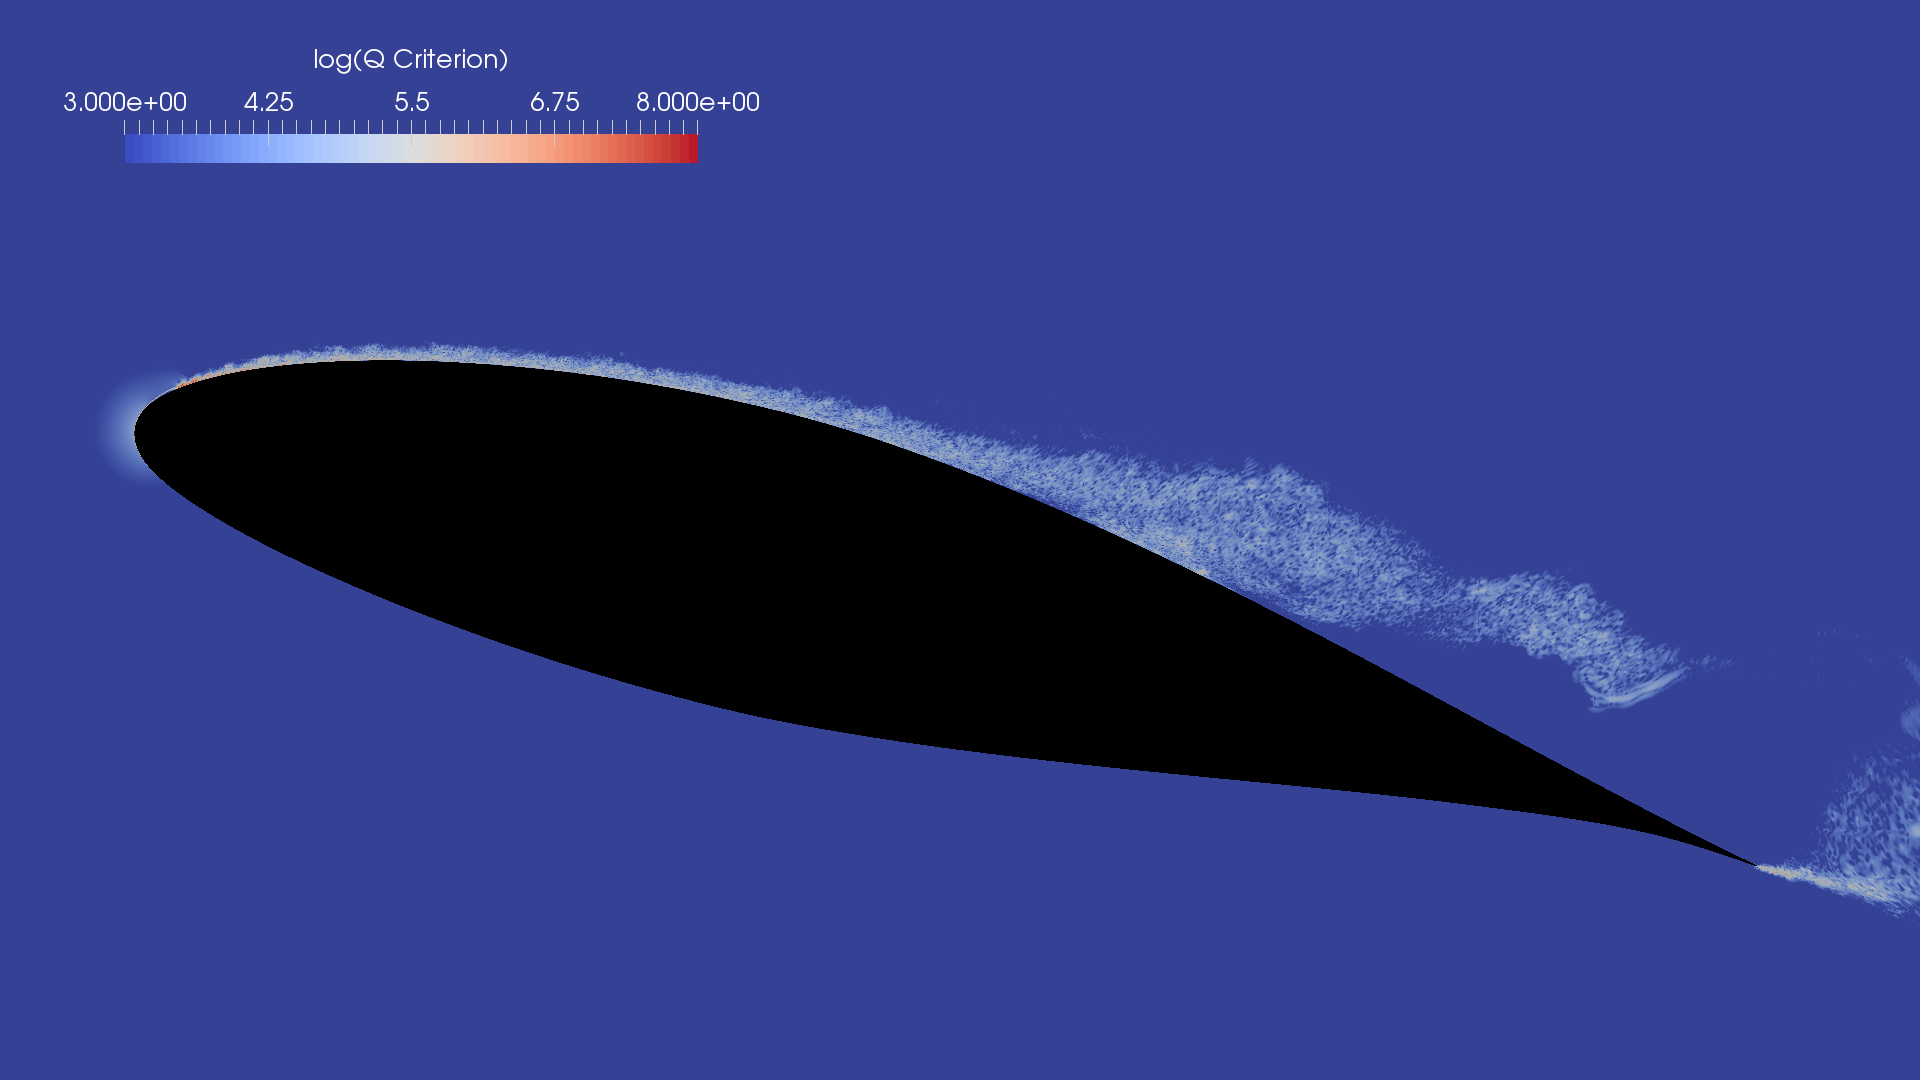
\includegraphics[width=.49\linewidth]{projects/2.3.6-NNSA/2.3.6.03-SNL-ATDM/SNL-ATDM-Nalu-Slice}
  \hfill
  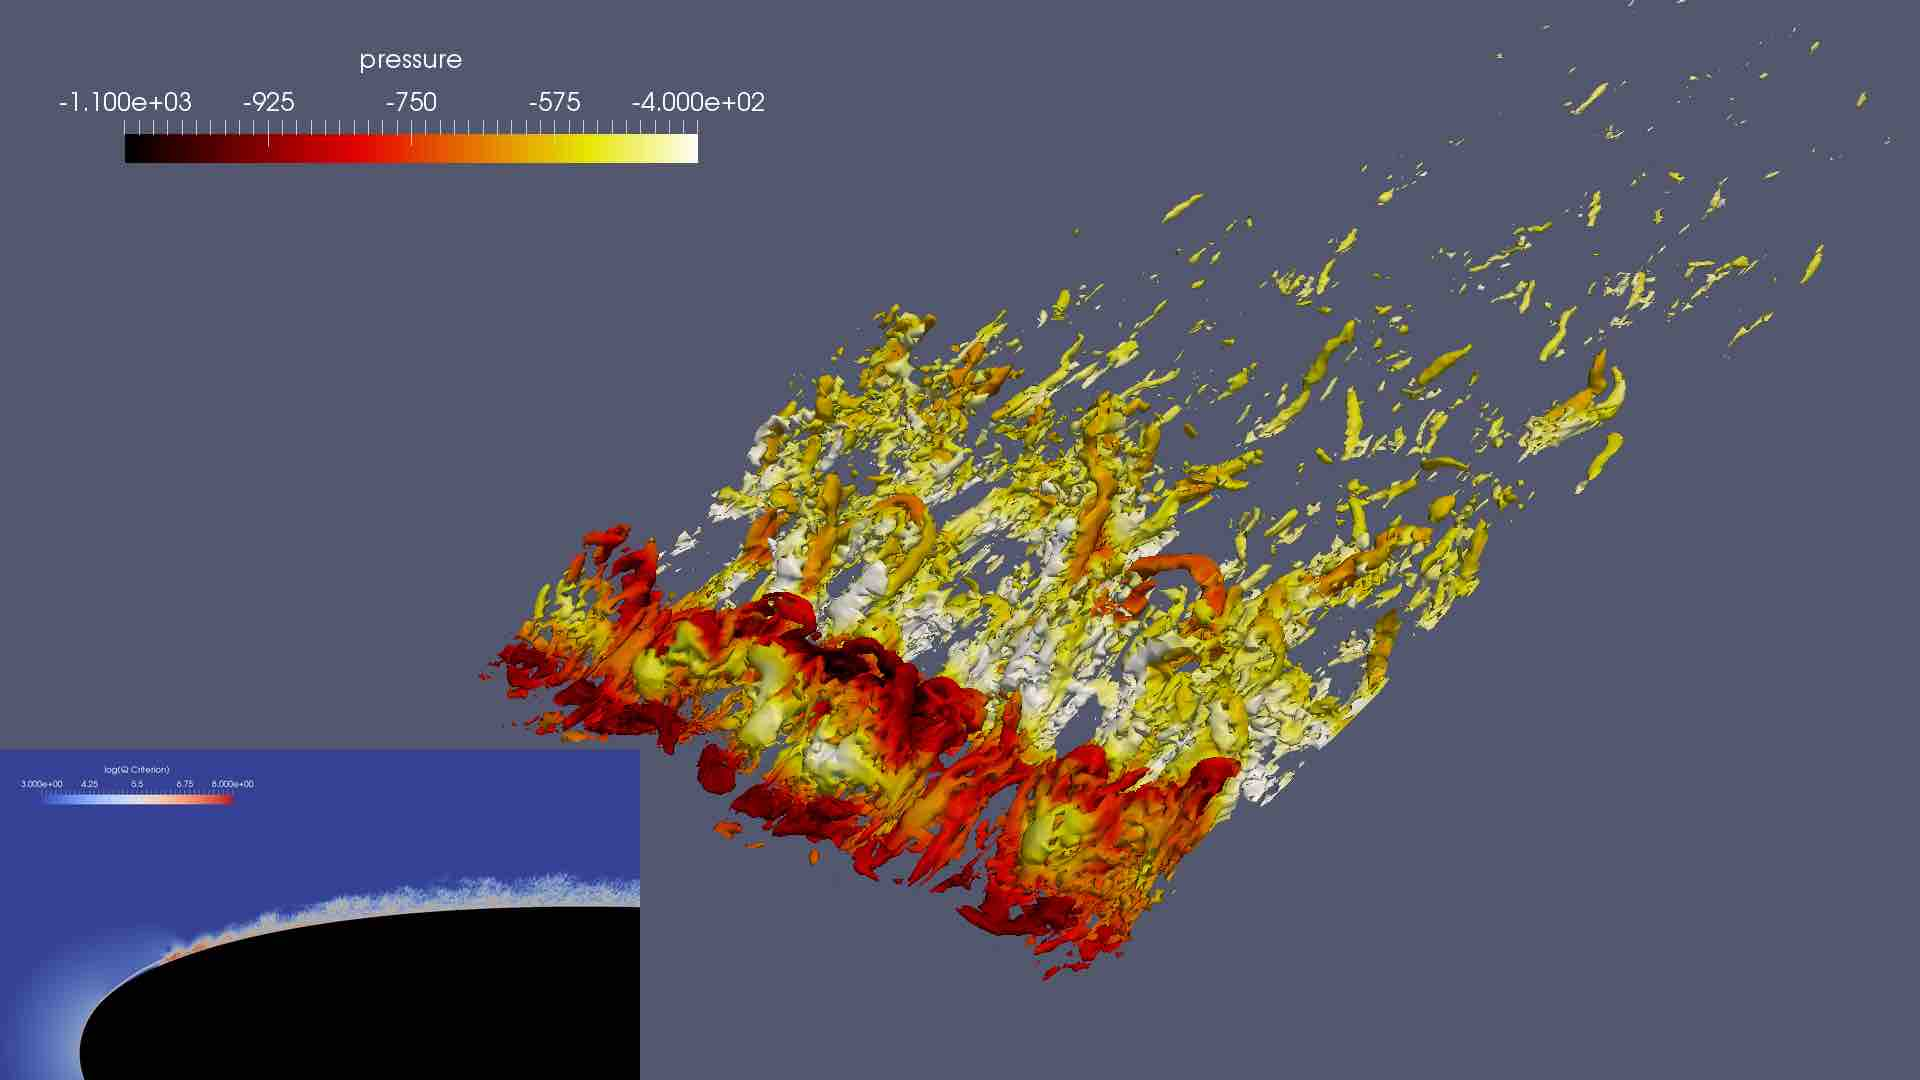
\includegraphics[width=.49\linewidth]{projects/2.3.6-NNSA/2.3.6.03-SNL-ATDM/SNL-ATDM-Nalu-Leading}
  \caption{
    Examples of an \emph{in situ} visualization of a Nalu simulation on 2560 processes of airflow over a wind turbine airfoil.
    At left: a cross-sectional slice through the airfoil along the direction of flow colored by Q criterion.
    %Higher values of Q criterion indicate the potential for vortex formation.
    At right: detail at the leading edge of the wind turbine airfoil.
    %The contours are at Q criterion value $10^7$, and are colored by the flow variable pressure.
  }
  \label{fig:SNL-ATDM-Vis-Nalu}
\end{figure}

Nalu \cite{Nalu} is a massively parallel unstructured low Mach flow code.
An adapter for Catalyst was developed for Nalu using the existing Seacas IOSS adapter for the Sierra framework to output unstructured mesh data to Catalyst.
Examples of \emph{in situ} visualization with Nalu are shown in Figure \ref{fig:SNL-ATDM-Vis-Nalu}.

Sparta \cite{Sparta} is a Sandia developed massively parallel DSMC (Direct Simulation Monte Carlo) code.
Sparta uses a unique hierarchical Cartesian grid structure to track simulation particle movement and interaction.
The Catalyst adapter implementation for Sparta uses shallow copy data structures to represent this hierarchy as an unstructured grid without forcing unnecessary copies of Sparta data structures.

\subparagraph{Data Compression}
Although the TuckerMPI compression library is already available as an open standalone git repository \cite{TuckerMPI-git}, we pursued three independent
approaches to integrate TuckerMPI compression with the \emph{in situ} technologies being developed in parallel: (1) modify Catalyst adapter, integrated 
with a miniFE demo example, to perform TuckerMPI compression (copy input data, create tensor data structures, perform compression over distributed data), 
(2) create a standalone ``TuckerWriter'' plugin for ParaView, packaged as a standalone shared object library (links appropriately with the separately 
built Tucker Library) that can be loaded from a ParaView GUI, and, (3) extend the SPARC Catalyst direct output branch to work alongside SPARC writer output. 
This extension allows Catalyst output from SPARC input decks that request output in a specific file format (CGNS), and will be used to construct test 
cases for TuckerMPI compression.

In addition to TuckerMPI integration with ParaView/Catalyst, we are also conducting R\&D to extend the capability to
compress unstructured non-rectilinear mesh data using functional tensor approximations. We are researching an approach whereby multi-variate data on an 
unstructured mesh is treated as a high-dimensional function (spatial dimensions, time), which may be approximated as a small sum of product of univariate 
functions. Encoding the univariate functions requires storing only a small number of function coefficients/parameters, resulting in large compression.  

\subparagraph{Algorithm Portability}
The SNL ATDM project is helping VTK-m run better on ASC platforms with multiple activities.
First, we are improving the parallel radix sorting operation in VTK-m.
Parallel sorting is a core component of many of our visualization algorithms.
Sorting helps us group common identifiers and conditions index sequences for fast searching.
Improving the performance of sort within the VTK-m framework implicitly improves the performance of many algorithms that already use it.
We are implementing a parallel radix sorting algorithm based on the work of Satish, et al. \cite{Satish2010}.
Our initial experiments indicate that the radix sort generally outperforms the default TBB sort algorithm typical data types.

Second, we are working to improve VTK-m's support vector instructions to improve performance on processors such as the Intel Xeon and Xeon Phi.
Compilers work to identify code loops where vectorization can be applied, but in VTK-m changes were required to help the compiler.
To enable vectorization across multiple complex data types, we are experimenting with loading values in blocks as we schedule an algorithm.
This allows the compiler to better vectorize worklet functions that are now accessing well behaved blocks of memory.
Given a sufficiently complex worklet, the benefit of better vectorization outweighs the overhead of maintaining blocks of values.

\noindent
{\tiny Sandia National Laboratories is a multimission laboratory managed and operated by National Technology \& Engineering Solutions of Sandia, LLC, a wholly owned subsidiary of Honeywell International Inc., for the U.S. Department of Energy's National Nuclear Security Administration under contract DE-NA0003525.
\par}
